\section{Overlapping industry spreads, 1980--2025}
Does a sign audit capture the practical difference between dependence models? We fixed a historical reconstruction before computing its endpoints. The source is the value-weighted monthly return table for the five US industry portfolios in Kenneth French's data library \cite{french}, September 2026 vintage. The sample comprises every January from 1980 through 2025. Each decision uses only earlier monthly rows in this vintage. Returns are decimal simple monthly returns. The audit uses historical inputs to measure configuration sensitivity; all calculated trades are hypothetical.

Set $w_0=(.2,\ldots,.2)^\top$ and $\lambda=3$. Three views each buy one industry (consumer, high technology or health) and sell manufacturing. The fifth sector is Other. All spreads have zero net investment. The manufacturing trade is $-(x_1+x_2+x_3)/3$. It cannot be recovered from separate view sign intervals. At each origin $\Sigma$ is the trailing 60-month sample covariance of sector returns, and each forecast in $q$ is the trailing 60-month mean spread return. The choice of total vs.\ excess returns cancels from each realized spread. We use the total-return covariance in the working prior. Unrestricted short sales and leverage are permitted in the main calculation.

For month $s$, form the realized spread minus its forecast using the 60 months preceding $s$. At each origin the sample covariance $V$ of the preceding 60 such errors supplies the working normalized variances $v_i=V_{ii}$. The share $h$ is the first hundredth in $[0,1]$ for which $V-(1-h)D\succeq0$, checked in rational arithmetic. This places the empirical error covariance in the ambiguity set. Realized forecast errors include return innovations. Their variances and correlations serve as a scale and a stress anchor, and do not identify errors in forecasts of latent expected returns. The cap varies from 0.30 to 0.85. We compare full dependence and all signed equicorrelation paths at the same $h$. The sensitivity calculation halves $h$.

\begin{table}[ht]
\centering\small
\caption{Certified widths of manufacturing tilts in percentage points. Columns 2--4 enclose medians across decision dates. Added width is computed within each date before taking its median. The last column counts dates permitting both trade directions under full and signed dependence.}
\begin{tabular}{lcccc}\toprule
January origins & Full width & Added over signed & Full, half share & Both signs (full/signed)\\\midrule
1980--1999 (20)&91.30--91.34&2.19--2.24&42.50--42.55&2/2\\
2000--2025 (26)&100.99--101.03&1.88--1.93&50.97--51.02&2/2\\
All (46)&93.79--93.83&2.06--2.10&45.54--45.59&4/4\\\bottomrule
\end{tabular}
\end{table}

Every year's sign classification agrees across the two stress families. The paired median width gap is positive in both periods. In January 1991 the full set permits a manufacturing overweight starting near 8.25 points, and the signed family starts near 19.09 points. The corresponding upper endpoints are about 129.95 and 121.61 points. Such sizes reflect the unconstrained optimizer and make the treatment of mandates consequential. Halving the dependence allowance cuts the full-sample median width to approximately 45.57 points and leaves one date admitting both signs. The annual windows overlap. All counts and medians describe this historical sequence; they are not estimates from 46 independent trials.

\paragraph{A manufacturing limit.}
As a post-design economic sensitivity, impose a 0--40\% manufacturing weight, with the other industries free and a unit net budget. The unconstrained tilt interval is clipped at $\pm20$ points. To see why, at fixed dependence the utility conditional on a specified manufacturing weight is a strictly concave quadratic in that weight after the other weights are optimized. Its peak is the original optimal weight, so restricting its domain clips the peak. Clipping is monotone, hence clips both sharp endpoints. Under this mandate the full feasible position is a single boundary weight in 32 of 46 years. The median extra width falls to zero. In eight years, five in the earlier period and three in the later period, the full set still adds over one point of feasible width beyond signed equicorrelation. This restriction applies to manufacturing only.

\begin{figure}[ht]
\centering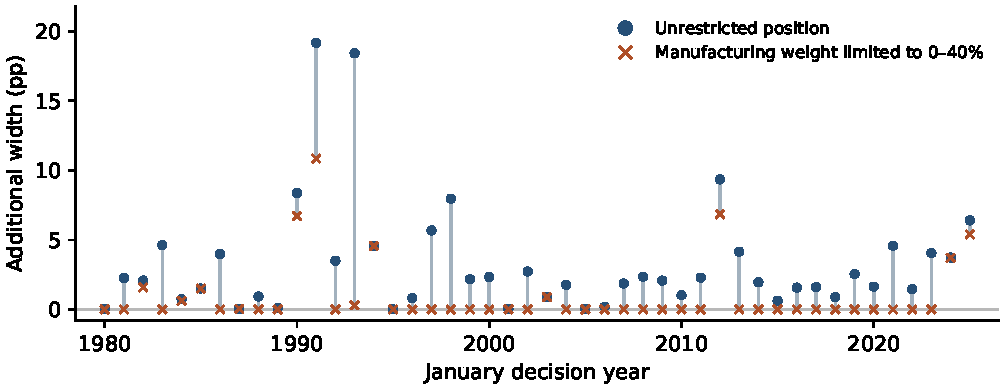
\includegraphics[width=.89\linewidth]{widths.pdf}
\caption{Within-year increase in the manufacturing tilt interval width when all admissible correlations replace signed common correlations. Markers use the midpoints of the endpoint enclosures. The capped comparison restricts only the manufacturing weight.}
\end{figure}

\paragraph{A fourth spread.}
In a separate post-design check we add Other minus manufacturing to the three spreads, recomputing all four forecast-error variances and the share at each origin. For the 92 signed manufacturing endpoints, the four individual-ellipsoid tests identify five minima and three maxima that require rank three in the dependent component. For instance, in January 1982 the upper manufacturing tilt is approximately 24.616 points, supported by the fourth ellipsoid. Its three remaining weighted residual lengths form a strict triangle. No two-factor covariance of the dependent component can attain that same allocation endpoint. Each of the other 84 endpoints admits a rank-at-most-two witness; all candidate exclusions were resolved with outward arithmetic. We classify those 84 endpoints without computing their magnitudes. This extension tests the dimension threshold on observed inputs in addition to the four-view construction.
